%   % !TEX root = ../../VIII,3_Rahmen-TeX_9-0.tex
%  
%   Signatur/Tex-Datei:	LH_37_05_161-162r
%   RK-Nr. 	57266_1			(_2 und _3 auf demselben Träger)
%   Überschrift: 	(keine)
%   Titel: 			Elaterium est causa imperfectionis in corporum concursu
%   Datierung:		März 1677, eigh.
%   WZ: 	Bl. 161, Nr. 803005
%   edlabels:			9 + 3 (Referenzierung)	
%   Diagramme: 		5					
%
%
%
\selectlanguage{ngerman}
\frenchspacing
%
\begin{ledgroupsized}[r]{120mm}
\footnotesize
\pstart
\noindent\textbf{Überlieferung:}
\pend
\end{ledgroupsized}
%
\begin{ledgroupsized}[r]{114mm}
\footnotesize
\pstart \parindent -6mm
\makebox[6mm][l]{\textit{L}}%
Konzept: LH~XXXVII~5, Bl.~161\textendash162.
Zwei~Blätter~2\textsuperscript{o}, die vermutlich ursprünglich einen Bogen bildeten;
Wasserzeichen auf Bl.~161;
Papierschaden an den Rändern mit geringfügigem Textverlust;
Papiererhaltungsmaßnahmen.
Zwei Seiten auf Bl.~161, eine Dreiviertelseite auf Bl.~162~r\textsuperscript{o};
Textfolge gemäß Blattzählung;
der untere Bereich von Bl.~162~r\textsuperscript{o} überliefert N.~\ref{57266_2}, Bl.~162~v\textsuperscript{o} überliefert N.~\ref{57266_3}.
\pend
\end{ledgroupsized}
%
\begin{ledgroupsized}[r]{114mm}
\footnotesize
\pstart
\parindent -6mm
\makebox[6mm][l]{\textit{E}}%
(tlw.) \cite{01056}\textsc{Fichant} 1994, S.~346\textendash352.
\pend%
\end{ledgroupsized}
%
%
%
\selectlanguage{latin}
\frenchspacing
% \newpage%
\vspace{8mm}
\pstart%
\normalsize%
\noindent%
\lbrack161~r\textsuperscript{o}\rbrack\
\pend
%
\count\Bfootins=1100%
\count\Afootins=1100%
\count\Cfootins=1100
\pstart
\noindent
\raggedleft
Martii 16\textlangle7\textrangle7
\pend
%
\vspace{2.0em} %%%%%%%%% Diagramm 1
\centerline{%
\includegraphics[width=0.45\textwidth]{%
gesamttex/edit_VIII,3/images/LH_37_05_161-162r_d1_161r.pdf%
}} 
\vspace{0.5em}
\centerline{%
\lbrack\textit{Fig.~1}\rbrack%
}
% \newpage%
\vspace{1.5em}
%
\pstart
\noindent
Sint duo corpora \edtext{aequalia%
\protect\index{Sachverzeichnis}{corpora aequalia}}{\lemma{}\Bfootnote{aequalia \textit{erg.}~\textit{L}}} 
%
\textit{A}, \textit{B} instructa atque armata vesicis%
\protect\index{Sachverzeichnis}{vesica} 
%
\edtext{aequ\textlangle ali\textrangle bus}{\lemma{}\Bfootnote{aequ\textlangle ali\textrangle bus \textit{erg.}~\textit{L}}} 
%
inflatis \textit{C}.\textit{D}.\ Ea concurrant
in  
\edtext{\textit{E}.\ ac}{\lemma{\textit{E}.}\Bfootnote{\textit{(1)}~impetu concursus \textit{(2)}~ac~\textit{L}}}
ponamus primo \textit{DB} quiescere, solumque \textit{AC} moveri.\pend
%
\pstart
Quaeritur incursu \textit{A} in \textit{B}, utrum 
\edtext{tantum comprimantur}
 {\lemma{tantum}\Bfootnote{\textit{(1)}~infletur \textit{(2)}~comprimantur~\textit{L}}}
vesicae,%
\protect\index{Sachverzeichnis}{vesica} an vero simul et corpus
\textit{B} nonnihil impellatur; si tantum inflatur vesica,%
\protect\index{Sachverzeichnis}{vesica} eousque donec major sit vis Elaterii%
\protect\index{Sachverzeichnis}{elaterium} aeris%
\protect\index{Sachverzeichnis}{aer}%
\protect\index{Sachverzeichnis}{vis elaterii aeris} quam ut
%[con] 
impulsu ipsius \textit{A} amplius comprimi possit, tunc vesica%
\protect\index{Sachverzeichnis}{vesica} se rursus ab altera 
\edtext{parte exonerans}
  {\lemma{parte}\Bfootnote{\textit{(1)}~detenden \textit{(2)}~de \textit{(3)}~exonerans~\textit{L}}}
in quantum impellitur, in tantum impellet ipsum \textit{B}, et cum eo simul abibit, sed initio tarde satis.
At \textit{A}, etsi  
%comm[unicatata]<unicata> 
\edtext{nonnihil communicata}{\lemma{nonnihil}\Bfootnote{\textit{(1)}~comminuat \textit{(2)}~communicata~\textit{L}}}
ipsi \textit{B} per vesicas%
\protect\index{Sachverzeichnis}{vesica} vi%
\protect\index{Sachverzeichnis}{vis} debilitatum
%[?] gestr.?
rursus assequetur, movetur
enim adhuc celerius quam \textit{B}, atque iterum comprimet  
\edtext{vesicas%
\protect\index{Sachverzeichnis}{vesica} ipsa}
  {\lemma{vesicas}\Bfootnote{\textit{(1)}~ipsas \textit{(2)}~ipsa~\textit{L}}}
separatione relaxatas, 
rursusque
novam vim%
\protect\index{Sachverzeichnis}{vis} ipsi \textit{B} communicabit, 
%[?] gestr.
idque tamdiu donec vis ipsi \textit{B} communicata, 
%[in qu] gestr. 
aequalis esse
incipiat ei quae restat ipsi \textit{A}, seu dimidia totius primae, tunc se non assequentur amplius, aequali enim 
celeritate%
\protect\index{Sachverzeichnis}{celeritas} ferentur, sed quae prioris dimidia est. Minime ergo hac arte efficiemus ut %
%
\edlabel{37_05_161-162r_3a}%
\edtext{}{% NEUER ABSATZ UND VARIANTEN – "XXX"
{\xxref%
{37_05_161-162r_3a}{37_05_161-162r_3b}}%
\lemma{uno}%
\Bfootnote{%
\textit{(1)}~quiescente alterum %
\textit{(2)}~\textit{A} quiescente moveatur \textit{B}. %
\textit{(a)}~Sed si omnis %
\textit{(b)}~Nec
\textit{L}%
}}%
uno \textit{A} quiescente moveatur tantum \textit{B}.
\pend
%
\pstart
Nec%
\edlabel{37_05_161-162r_3b}
%
proinde admittendum est,
\edtext{ut tantum}
  {\lemma{ut}\Bfootnote{\textit{(1)}~solum impellatur Elaterium  \textit{(2)}~tantum~\textit{L}}}
comprimatur vesica,%
\protect\index{Sachverzeichnis}{vesica} non vero 
\edtext{et impellatur}
  {\lemma{et}\Bfootnote{\textit{(1)}~comprimatur Elaterium  \textit{(2)}~impellatur~\textit{L}}}
corpus \textit{B}. Itaque \textit{A} impingente in \textit{B}, patet %
obstaculum\protect\index{Sachverzeichnis}{obstaculum} quod ipsi \textit{A} objicitur duobus modis tolli
uno si impellatur \textit{B}, altero si comprimantur vesicae%
\protect\index{Sachverzeichnis}{vesica} \edtext{\lbrack\textit{C}, \textit{D}\rbrack.}{%
\lemma{}%
\Bfootnote{%
\textit{ED} %
\textit{L ändert Hrsg.}%
}}
%
Et primum corpus \textit{B}, impelli potest, ea conditione
ut tantum decedat celeritati%
\protect\index{Sachverzeichnis}{celeritas} 
\edtext{ipsius \textit{A}}
  {\lemma{ipsius}\Bfootnote{\textit{(1)}~\textit{E}, \textit{(2)}~\textit{A}~\textit{L}}}
quantum ipsi datur, cum ergo posito \textit{A} et \textit{B} aequales,
conatum accipiat \textit{B} eundi%
\protect\index{Sachverzeichnis}{conatus eundi} cum \textit{A}, 
\edtext{sed celeritate}
  {\lemma{sed}\Bfootnote{\textit{(1)}~ea celeritate qu  \textit{(2)}~celeritate~\textit{L}}}
prioris dimidia, et \textit{A} etiam, ideo percussionem\protect\index{Sachverzeichnis}{percussio} seu mutationem,\protect\index{Sachverzeichnis}{percussio} in se recipiunt vesicae,%
\protect\index{Sachverzeichnis}{vesica} 
quantum enim ipsi \textit{A} detractum est, seu quantum
sensit obstaculum,%
\protect\index{Sachverzeichnis}{obstaculum} tanta est %
percussio.\protect\index{Sachverzeichnis}{percussio} 
\pend
\pstart
Percussio%
\protect\index{Sachverzeichnis}{percussio} quippe sine obstaculo%
\protect\index{Sachverzeichnis}{obstaculum} nulla est. Est
ergo 
%[per] 
 tanta quanta est diminutio virium%
\protect\index{Sachverzeichnis}{diminutio virium} ipsius \textit{A}, 
%
\edtext{seu dimidium}{%
\lemma{seu}%
\Bfootnote{%
\textit{(1)}~quanta %
\textit{(2)}~ dimidium %
\textit{L}%
}}
%
primae vis.
Ea %
percussio\protect\index{Sachverzeichnis}{percussio} recipitur in vesicis, et vesicis%
\protect\index{Sachverzeichnis}{vesica} se rursus 
%[de] 
aperientibus 
%[tum] oder [tam] 
dimidium huius dimidii 
%
\edtext{impe\lbrack nd\rbrack itur}{%
\lemma{}%
\Bfootnote{%
impellitur %
\textit{L ändert Hrsg.}%
}}
%
repellendo \textit{A}, alterum dimidium propellendo \textit{B}. Itaque \textit{A} perget $\frac{1}{4}$ta parte suae celeritatis primae, 
\textit{B} vero tribus quartis. Verum hoc et 
\edtext{experientiae%
\protect\index{Sachverzeichnis}{experientia} et rationi%
\protect\index{Sachverzeichnis}{ratio}}
  {\lemma{experientiae}\Bfootnote{et \textit{(1)}~rationis  \textit{(2)}~rationi~\textit{L}}}
contrarium. Experientiae%
\protect\index{Sachverzeichnis}{experientia}
ut notum. Rationi%
\protect\index{Sachverzeichnis}{ratio} vero, quia ita revera plus virium%
\protect\index{Sachverzeichnis}{vis} producitur, quam erat in producente, nempe
%[no] 
post ictum%
\protect\index{Sachverzeichnis}{ictus} motus ipsius \textit{A}, motus ipsius \textit{B}, qui simul aequales primo motui ipsius \textit{A}, et praeterea vis vesicis%
\protect\index{Sachverzeichnis}{vesica} 
percussione%
\protect\index{Sachverzeichnis}{percussio} communicata. Aliter ergo ratiocinandum et sic quidem. 
\pend
\pstart
Corpus \textit{A} impingens in \textit{B},
duo habet %
obstacula\protect\index{Sachverzeichnis}{obstaculum} alternativa, unum molem%
\protect\index{Sachverzeichnis}{molis} corporis \textit{B}, alterum, 
\edtext{Elaterium%
\protect\index{Sachverzeichnis}{elaterium} vesicarum,}
  {\lemma{Elaterium}\Bfootnote{\textit{(1)}~ipsius  \textit{(2)}~vesicarum,~\textit{L}}}
itaque
%[dimid] 
corpus duo habet %
obstacula,\protect\index{Sachverzeichnis}{obstaculum} unum ipsius 
%[Ela] 
vesicae, quae parum initio comprimenda est, alterum totius corporis
\textit{B} propellendi. Obstaculum vesicae parvum est,  
\edtext{corporis \textit{B} magnum,}
   {\lemma{}\Bfootnote{corporis \textbar\ \textit{B} \textit{erg.}~\textbar\ magnum,~\textit{L}}} nam si corpus 
%[p] 
\textit{B} propellendum est, amittit corpus 
\textit{A} dimidium celeritatis%
\protect\index{Sachverzeichnis}{celeritas} suae, si vero \edtext{vesica%
\protect\index{Sachverzeichnis}{vesica} parum comprimitur,}
{\lemma{}\Bfootnote{vesica \textbar\ parum \textit{erg.}~\textbar\ comprimitur~\textit{L}}} 
 tantum solummodo amittit quantum vesicae%
\protect\index{Sachverzeichnis}{vesica} parum compressae
Elaterium%
\protect\index{Sachverzeichnis}{elaterium} absumit, quod est exiguum. Patet ergo non amplius amittere debere virium%
\protect\index{Sachverzeichnis}{vis} corpus \textit{A}, quam exiguo %
obstaculo\protect\index{Sachverzeichnis}{obstaculum}
%[??] 
impendit. Quaeritur  
\edtext{tamen an illam}
  {\lemma{tamen}\Bfootnote{an \textit{(1)}~illum  \textit{(2)}~illam~\textit{L}}}
vim%
\protect\index{Sachverzeichnis}{vis} impendat soli tantum Elaterio,%
\protect\index{Sachverzeichnis}{elaterium} an vero toti 
\edtext{corpori et}
  {\lemma{corpori}\Bfootnote{\textit{(1)}~et si toti  \textit{(2)}~et~\textit{L}}}
Elaterio%
\protect\index{Sachverzeichnis}{elaterium} simul. Si soli Elaterio,%
\protect\index{Sachverzeichnis}{elaterium} tunc patet ex 
 \edtext{pluribus solum}
    {\lemma{}\Bfootnote{pluribus \ \textbar \ debilibus \textit{gestr.}\ \textbar\ solum~\textit{L}}}
cedere debilissimum; et reliqua
omnino non. Huc pertinet experimentum de pluribus Elateriis%
\protect\index{Sachverzeichnis}{elaterium} se comprimentibus,%
\protect\index{Sachverzeichnis}{experimentum de pluribus Elateriis se comprimentibus} ex quibus videndum 
 \edtext{an debile}
    {\lemma{}\Bfootnote{an \ \textbar \ unum \textit{gestr.}\ \textbar\ debile~\textit{L}}}
cedat solum. Si 
\edtext{vero et}
  {\lemma{vero}\Bfootnote{\textit{(1)}~totum \textit{(2)}~et~\textit{L}}}
corpus et %
elaterium\protect\index{Sachverzeichnis}{elaterium} exiguam illam %
vim\protect\index{Sachverzeichnis}{vis} reciperent, quaestio rursus est,
quanam proportione. Videtur 
\edtext{enim quaedam}{\lemma{}\Bfootnote{enim \ \textbar \ nova \textit{gestr.}\ \textbar\ quaedam~\textit{L}}}  
oriri replicatio,%
\protect\index{Sachverzeichnis}{replicatio} quod in quantum corpus cedit,
in tantum etiam %
elaterio\protect\index{Sachverzeichnis}{elaterium} decedit.
%[se] 
Exactissime haec discutienda, patet enim niti principiis mere
metaphysicis,%
\protect\index{Sachverzeichnis}{principium metaphysicum} et praeterea experimentis%
\protect\index{Sachverzeichnis}{experimentum} posse determinari. Sed ponendo solum 
\edtext{Elaterium vesicarum,%
\protect\index{Sachverzeichnis}{Elaterium vesicae}}
  {\lemma{Elaterium}\Bfootnote{\textit{(1)}~recipi \textit{(2)}~vesicarum,~\textit{L}}}
quippe debilius corpore%
\protect\index{Sachverzeichnis}{corpus debilius} cedere, tunc, utique in quantum compressae vesicae,%
\protect\index{Sachverzeichnis}{vesica} in tantum, rursus se
exonerabunt, et 
%[agent?] [agent?] 
agent tum in \textit{A}, tum in \textit{B}, in quantum agent in \textit{A}, ab ipso \textit{A} repellentur,
ne mutua actione%
\protect\index{Sachverzeichnis}{actio mutua} destruatur vis,%
\protect\index{Sachverzeichnis}{vis} in quantum agent in \textit{B}, ipsum \textit{B}, quippe non resistens 
\edtext{propellent. Ut}
  {\lemma{propellent.}\Bfootnote{\textit{(1)}~In quantum vis Elastica
ab \textit{A} repulsa est,  \textit{(2)}~Vis Elastica repellitur ab \textit{A} eo modo \textit{(3)}~Ut~\textit{L}}}
consideretur, quomodo vis Elastica repellitur
%[?] 
\edtext{ab \textit{A}, ponamus}
  {\lemma{ab \textit{A},}\Bfootnote{\textit{(1)}~considerandum est quid fiat, si Elaterium aliquod opponat se corpori in ipsum prementi, 
  \textbar\ tunc \textit{streicht Hrsg.}\ \textbar\
  si fortius sit corpus quam vis Elaterii, \textit{(a)}~ne \textit{(b)}~non putandum est, \textit{(aa)}~a vi prementis \textit{(bb)}~mob
\textit{(cc)}~mutuo nixu
  \textit{(2)}~ponamus~\textit{L}}}
corpus grave quod Elaterio se aperire conanti sit impositum,%
\protect\index{Sachverzeichnis}{grave impositum Elaterio se aperire conanti} est quaedam determinata in gravi%
\protect\index{Sachverzeichnis}{grave}
vis descendendi,%
\protect\index{Sachverzeichnis}{vis descendendi} item alia in Elaterio%
\protect\index{Sachverzeichnis}{elaterium} se aperiendi.%
\protect\index{Sachverzeichnis}{vis se aperiendi} Ponamus eas duas \edtext{vi\lbrack{}re\rbrack{}s%
\protect\index{Sachverzeichnis}{vis}}{%
\lemma{}%
\Bfootnote{%
vis %
\textit{L ändert Hrsg.}%
}}
 esse aequales utique neque
%
elaterium\protect\index{Sachverzeichnis}{elaterium} se aperiet, neque %
grave\protect\index{Sachverzeichnis}{grave} descendet, non tamen ideo  
\edtext{quicquam de vi%
\protect\index{Sachverzeichnis}{vis}}
  {\lemma{quicquam}\Bfootnote{de \textit{(1)}~motu perdetur \textit{(2)}~vi~\textit{L}}}
perdetur,
ea enim manebit, sed nec de
\edtext{motu%
\protect\index{Sachverzeichnis}{motus} perdetur, quia}
   {\lemma{}\Bfootnote{motu \textbar\ perdetur \textit{erg.}~\textbar\ , quia~\textit{L}}}
corpora 
\edtext{insensibilia%
\protect\index{Sachverzeichnis}{corpus insensibile}}
  {\lemma{}\Bfootnote{insensibilia \textit{erg.}~\textit{L}}}
eam vim causantia%
\protect\index{Sachverzeichnis}{corpora insensibilia vim causantia} ictibus%
\protect\index{Sachverzeichnis}{ictus} suis repellentur seu reflectentur.
Quando vero motus non est aliunde, 
% <?>
sed in ipsis corporibus\lbrack,\rbrack\ tunc ambo repelli necesse est, et quidem pro virium%
\protect\index{Sachverzeichnis}{vis} ratione variis modis. Sed omnibus examinatis res puto eo tandem redibit, ut ambo corpora procedant in eandem 
enim quam ante lineam, dimidia celeritate%
\protect\index{Sachverzeichnis}{celeritas} ut supra.
\pend
%
\vspace{2.0em} %%%%%%%%% Diagramm 2
\centerline{%
\includegraphics[width=0.33\textwidth]{%
gesamttex/edit_VIII,3/images/LH_37_05_161-162r_d2_161r.pdf%
}} 
\vspace{0.5em}
\centerline{%
\lbrack\textit{Fig.~2}\rbrack%
}
\newpage%
%\vspace{1.5em}
%
\pstart
\hspace{1mm}\hspace{-1mm}% Trick, weil \edlabel nicht zu \par-Beginn sein darf
\edlabel{37_05_161-162r_1a}%
\edtext{}{% A-Footnote – Diagramm und Rechnung
{\xxref%
{37_05_161-162r_1a}{37_05_161-162r_1b}}%
\lemma{}%
\Afootnote{\textit{Am Rand}: %
\protect\begin{center} 
\protect\includegraphics[width=0.4\textwidth]{gesamttex/edit_VIII,3/images/LH_37_05_161-162r_d3_161r.pdf}\\
\vspace{0.5em}
\protect\centerline{\lbrack\textit{Fig.~3}\rbrack\textsuperscript{\lbrack a\rbrack}}
\protect\centering 
\vspace{-1.0em}
\protect\begin{gather*}
	\protect\begin{array}{cc}
		\textit{\scriptsize{2}}a\textit{\scriptsize{1}}b. & \textit{\scriptsize{1}}a\textit{\scriptsize{2}}B\\
		\textup{celeritas}&\textup{corpus}\\
		a & A \\
		b & B
	\protect\end{array}\\
	4aB + 2B \sqcap 6
\protect\end{gather*}
\protect\end{center}
%Marginalienapparat:
{\footnotesize \textsuperscript{\lbrack a\rbrack} \lbrack\textit{Fig.~3}\rbrack: Ein gestrichener Entwurf zum Diagramm wird nicht wiedergegeben.%
}%
\newline%
}}%
Sed omissis vesicis%
\protect\index{Sachverzeichnis}{vesica} sumamus corpora Elastica dura,%
\protect\index{Sachverzeichnis}{corpus elasticum durum} cum 
\edtext{scilicet Elateria%
\protect\index{Sachverzeichnis}{elaterium}}
  {\lemma{scilicet}\Bfootnote{\textit{(1)}~non differt a corpore ipso, \textit{(2)}~Ela \textit{(3)}~Elasti \textit{(4)}~Elateria~\textit{L}}}
non differunt a corporibus. Considerandum est
ergo duobus corporibus Elasticis duris%
\protect\index{Sachverzeichnis}{corpus elasticum durum} 
\edtext{\textit{A}.\textit{B}.}
  {\lemma{}\Bfootnote{\textit{A}.\textit{B}. \textit{erg.}~\textit{L}}}
 concurrentibus, duplicem 
\edtext{vim%
\protect\index{Sachverzeichnis}{vis} exerceri,}
  {\lemma{vim}\Bfootnote{\textit{(1)}~esse in natu  \textit{(2)}~na \textit{(3)}~exerceri,~\textit{L}}}
unam in propellenda
\edtext{corpora eo}{\lemma{}\Bfootnote{corpora\ \textbar \ versus \textit{E} \textit{gestr.}\ \textbar\ eo~\textit{L}}}
modo
quo leges ferent, 
\edtext{alter\lbrack{}a\rbrack{}m}{\lemma{}\Bfootnote{alterum\textit{\ L ändert Hrsg.}}}
in ea dissipanda atque
\edtext{frangenda. \edlabel{37_05_161-162r_2a}Cumque}{\lemma{frangenda}\Bfootnote{\textit{(1)}~, is \textit{(2)}~, idem enim est vim actricem exerc \textit{(3)}~. Cumque~\textit{L}}}
%
\edtext{}{% A-Footnote – "NB"
{\xxref%
{37_05_161-162r_2a}{37_05_161-162r_2b}}%
\lemma{}%
\Afootnote{\textit{Am Rand}: NB}}%
nulla sit ratio cur %
vis actrix\protect\index{Sachverzeichnis}{vis actrix} 
exerat\edlabel{37_05_161-162r_1b}
%
se potius in motum corporum 
\edtext{particularem%
\protect\index{Sachverzeichnis}{motus particularis}}
  {\lemma{particularem}\Bfootnote{\textit{erg.}~\textit{L}}}, 
%
quam in dissipationem%
\protect\index{Sachverzeichnis}{dissipatio}
\edtext{quae esset}
  {\lemma{quae}\Bfootnote{\textit{(1)}~erit  \textit{(2)}~esset~\textit{L}}}
causa quietis,%
\protect\index{Sachverzeichnis}{quies} id est motus corporum cum tota%
\edlabel{37_05_161-162r_2b}
%
massa communis.%
\protect\index{Sachverzeichnis}{motus communis cum tota massa} 
Hinc dimidia vis impendetur in corporum 
%[f] 
rupturam.%
\protect\index{Sachverzeichnis}{ruptura} Et ideo dimidia 
\edtext{semper vis erit}
  {\lemma{semper}\Bfootnote{vis \textit{(1)}~esse  \textit{(2)}~erit~\textit{L}}}
ipsa 
%[†] 
vis percussionis.%
\protect\index{Sachverzeichnis}{vis percussionis} Ponendo 
\edtext{ergo corporum}
  {\lemma{ergo}\Bfootnote{\textit{(1)}~corpus dimidiam sentire vim  \textit{(2)}~duo corpora \textit{(3)}~corporum~\textit{L}}}
molem%
\protect\index{Sachverzeichnis}{molis} dimidiam
ictus vim%
\protect\index{Sachverzeichnis}{vis ictus} sentire, manifeste patet 
\edtext{cur impingens}
  {\lemma{cur}\Bfootnote{\textit{(1)}~unum alio celerius proceda \textit{(2)}~impingens~\textit{L}}}
quiescat, alterum vero procedat eadem
vi.%
\protect\index{Sachverzeichnis}{vis} Nempe ictus %
corpus durum\protect\index{Sachverzeichnis}{corpus durum} totum contusit, ita ut se inflectat 
\edtext{longius, quam impellens}
  {\lemma{longius,}\Bfootnote{quam \textit{(1)}~alter \textit{(2)}~impellens~\textit{L}}}
persequitur, uti
%
lamina\protect\index{Sachverzeichnis}{lamina} percussa longius se flectit, quam impellens, quod secus est in mollibus, ut 
\edtext{vesicis. Hinc}
  {\lemma{vesicis}\Bfootnote{\textit{(1)}~, in \textit{(2)}~. Hinc~\textit{L}}}
dimidia vi in 
%[cor]
\textlangle cor\textrangle poris massam%
\protect\index{Sachverzeichnis}{massa} impensa, altera dimidia restabit in corporibus et ambo pergent 
\edtext{celeritate%
\protect\index{Sachverzeichnis}{celeritas} quae}
  {\lemma{celeritate}\Bfootnote{\textit{(1)}~prioris \textit{(2)}~quae~\textit{L}}}
prioris
\textlangle est\textrangle\
quarta pars, quia id quod nunc movetur, prioris duplum, ita enim motus qui nunc in ipsis est prioris dimidius \textlangle est.\textrangle\
Cum ergo \textit{A} eat celeritate $\frac{1}{4}$ et \textit{B} celeritate $\frac{1}{4}$  %
Elaterium\protect\index{Sachverzeichnis}{elaterium} ipsorummet 
%[??] 
se repellentium vi%
\protect\index{Sachverzeichnis}{vis} $\frac{1}{2}$, aequaliter
eam dividet quia eor\textlangle um\textrangle\ vires%
\protect\index{Sachverzeichnis}{vis} sunt aequales, et ita corpus \textit{A} 
\edtext{celeritate ut $\frac{1}{4}$ repelletur,}
  {\lemma{celeritate ut $\frac{1}{4}$}\Bfootnote{\textit{(1)}~recedens \textit{(2)}~ repelletur,~\textit{L}}}
cumque simul celeritate%
\protect\index{Sachverzeichnis}{celeritas} 
\lbrack161~v\textsuperscript{o}\rbrack\
ut $\frac{1}{4}$ veniat\lbrack,\rbrack\
%
\edtext{quiescet\lbrack;\rbrack\ corpus}{%
\lemma{}%
\Bfootnote{%
quiescet \textbar\ \textit{A} \textit{erg., streicht Hrsg.}~\textbar\ corpus \textit{L}%
}}
vero \textit{B}, quod antea celeritate 
ut $\frac{1}{4}$ movebatur, nunc celeritate $\frac{1}{4}$\lbrack,\rbrack\
movebitur celeritate%
\protect\index{Sachverzeichnis}{celeritas} $\frac{1}{2}$. Verum sic quoque non obtinemus quaesitum.
\pend
\pstart
Videtur pro certo habendum ictum%
\protect\index{Sachverzeichnis}{ictus} qui 
%[ap] 
ex corporum appropinquatione oritur%
\protect\index{Sachverzeichnis}{ictus ex appropinquatione corporum} esse
eundem, quodcunque 
%[??] 
corporum moveatur aut quiescat
nec videtur referre 
egone % FI: egone 
in parietem%
\protect\index{Sachverzeichnis}{paries}
impingam magna celeritate,%
\protect\index{Sachverzeichnis}{celeritas} an paries%
\protect\index{Sachverzeichnis}{paries} in me.
\pend
\pstart
Efficit autem hic ictus,%
\protect\index{Sachverzeichnis}{ictus} ut corpora a se invicem
resilire conentur\lbrack,\rbrack\ % FI conentur,
quae %
vis resiliendi\protect\index{Sachverzeichnis}{vis resiliendi} tanta est, quanta est vis concursus.%
\protect\index{Sachverzeichnis}{vis concursus} 
\pend 
\pstart
Praeterea corpora 
ambo post concursum%
\protect\index{Sachverzeichnis}{concursus} pergunt eadem qua ante vi.%
\protect\index{Sachverzeichnis}{vis}
Vis autem e concursu orta%
\protect\index{Sachverzeichnis}{vis orta e concursu} ea a
se invicem repellit, in reciproca ratione molium%
\protect\index{Sachverzeichnis}{molis} et celeritatum%
\protect\index{Sachverzeichnis}{celeritas}
id est si aequalia sint aequali. Itaque si corpora 
\edtext{duo sint aequalia et}
{\lemma{duo}\Bfootnote{\textit{(1)}~aequaliter \textit{(2)}~aequalia, quorum unum in alterum imping \textit{(3)}~sint aequalia et~\textit{L}}}
unum impingat in
aliud quiescens, % FI: quiescens,
tunc  
\edtext{ipsum quiescens propelletur}{\lemma{ipsum}\Bfootnote{quiescens \textit{(1)}~impelletur \textit{(2)}~propelletur~\textit{L}}}
dimidia %
vi%
\protect\index{Sachverzeichnis}{vis} impellentis et dimidia vi resilitionis,%
\protect\index{Sachverzeichnis}{vis resilitionis} id est tota 
vi impellentis, at % FI: et fehlt 
impingens progredietur dimidia vi sua, regredietur, % FI: Komma fehlt
dimidia resilitionis.%
\protect\index{Sachverzeichnis}{vis resilitionis}
Et ita
impulsum ibit celeritate impellentis. Tantum in eo est difficultas, quod hoc modo videtur reapse multiplicari vis,%
\protect\index{Sachverzeichnis}{vis} tametsi in effectu 
%<††> 
\edtext{destruendo fiat,}
  {\lemma{destruendo}\Bfootnote{\textit{(1)}~effici \textit{(2)}~fiat,~\textit{L}}}
ut multiplicatio non sentiatur, % FI: sentiatur; 
\edtext{nimirum vis}
  {\lemma{nimirum}\Bfootnote{\textit{(1)}~vis a concursu \textit{(2)}~vis~\textit{L}}}
ictus%
\protect\index{Sachverzeichnis}{vis ictus} seu concursus ab appropinquatione,%
\protect\index{Sachverzeichnis}{vis concursus ab appropinquatio}%
\protect\index{Sachverzeichnis}{concursus ab appropinquatio} % FI: Komma fehlt
separata est a vi quae corpora promovet, % FI: Komma fehlt
et tamen
utraque separatim orta est ex una tantum singulis aequali. Quare si vis illa resiliendi%
\protect\index{Sachverzeichnis}{vis resiliendi} orta diverti
posset separatimque ab ipsa ferente%
\protect\index{Sachverzeichnis}{vis ferens} 
%<exce> 
exerceri,
\edtext{haberetur effectus}
  {\lemma{haberetur}\Bfootnote{\textit{(1)}~vis \textit{(2)}~effectus~\textit{L}}}
major causa.%
\protect\index{Sachverzeichnis}{effectus major causa} Verum
enim 
\edtext{vero responderi} % FI: Verum enim vero fehlt
  {\lemma{vero}\Bfootnote{\textit{(1)}~haec frustra dicendum est contingere \textit{(2)}~responderi~\textit{L}}}
potest fortasse impossibile esse ut separentur. Mihi
tamen ut verum fatear suspecta 
est haec ratiocinatio. Certum enim est vim%
\protect\index{Sachverzeichnis}{vis} augere saltem 
\edtext{aliquo tempore,}
  {\lemma{aliquo}\Bfootnote{\textit{(1)}~momento \textit{(2)}~tempore,~\textit{L}}}
quod implicare videtur. 
\pend
\pstart
Praeterea experimentis ex sono%
\protect\index{Sachverzeichnis}{sonus} sumtis%
\protect\index{Sachverzeichnis}{experimentum ex sono sumtum} dijudicandum est, utrum
tanta sit vis 
\edtext{percussionis%
\protect\index{Sachverzeichnis}{vis percussionis} cum}
  {\lemma{percussionis}\Bfootnote{\textit{(1)}~cum duo corpora ae \textit{(2)}~cum~\textit{L}}}
%<qu> 
corpus motum incurrit in aequale quiescens,
et cum duo corpora aequaliter 
%<?> 
mota sibi %
\edlabel{37_05_161-162r_4a}%
\edtext{}{{\xxref{37_05_161-162r_4a}{37_05_161-162r_4b}}%
{\lemma{occurrunt.}\Bfootnote{\textit{(1)}~Dicere autem  \textit{(2)}~Non licet \textit{(3)}~Quid~\textit{L}}}}%
occurrunt.
\pend
\newpage
\count\Bfootins=1000%
\count\Afootins=1200%
\count\Cfootins=1000
\pstart
Quid\edlabel{37_05_161-162r_4b} si dicamus totam vim quidem in percussionem%
\protect\index{Sachverzeichnis}{percussio} insumi, et ita corpora aequaliter repelli,
sed ne id fiat novam 
\edtext{liquidi circumfusi%
\protect\index{Sachverzeichnis}{liquidum circumfusum}}
  {\lemma{liquidi}\Bfootnote{\textit{(1)}~circumeuntis \textit{(2)}~circumfusi~\textit{L}}}
vim%
\protect\index{Sachverzeichnis}{vis} efficere, quae faciat
continuari
praeterea motum. Tunc rem dicemus experimentis%
\protect\index{Sachverzeichnis}{experimentum} contrariam, quia 
\edtext{corpus quod subito}{\lemma{corpus}\Bfootnote{\textit{(1)}~semel \textit{(2)}~quod subito~\textit{L}\hspace{-2mm}}}
manu in
quiete ponitur, hoc modo redingruente ictu%
\protect\index{Sachverzeichnis}{ictus} materiae circumfusae%
\protect\index{Sachverzeichnis}{materia circumfusa} 
\edtext{abriperetur. Liquidum%
\protect\index{Sachverzeichnis}{liquidum}}
  {\lemma{abriperetur}\Bfootnote{\textit{(1)}~, ut liquidum \textit{(2)}~. Liquidum~\textit{L}}}
baculo%
\protect\index{Sachverzeichnis}{baculus} agitatum corpus in eo natans in quiete collocatum, nihilominus iterum post quietem arripit. Sed secus
est, si non nisi ab ipsius natantis vi agitaretur, tunc enim 
%<liqu> 
natante in quiete posito liquidum%
\protect\index{Sachverzeichnis}{liquidum} id 
ipsum postea non abripiet.
\pend
\pstart
%Ex 
Experimento%
\protect\index{Sachverzeichnis}{experimentum} videtur definiri posse, an tantundem resonent duo corpora aequalia aequali motu 
%
\edtext{concurrentia,%
\protect\index{Sachverzeichnis}{corpora aequalia aequali motu concurrentia} ac si}{\lemma{concurrentia,}\Bfootnote{\textit{(1)}~ac concurrentia vi aequali duplo \textit{(2)}~ac si~\textit{L}}}
%
unum in alterum \edtext{quiescens}{\lemma{}\Bfootnote{quiescens \textit{erg.}~\textit{L}}}
%
duplo celeriore ictu \edlabel{37_05_161-162r_5a}%
\edtext{}{{\xxref{37_05_161-162r_5a}{37_05_161-162r_5b}}%
{\lemma{ferretur.}\Bfootnote{\textit{(1)}~Videtur dicendum totam vim quidem sentire corpora per ictum, et  \textit{(2)}~Non~\textit{L}}}}%
ferretur.
\pend
\pstart
Non\edlabel{37_05_161-162r_5b} videtur possibile ut corpora totam vim%
\protect\index{Sachverzeichnis}{vis} sentiant per ictum,%
\protect\index{Sachverzeichnis}{ictus} et ita complicentur, nam si satis essent magna, et ita vim Elaterio%
\protect\index{Sachverzeichnis}{elaterium} totam continerent, et praeterea moverentur, possemus machinari motum perpetuum,%
\protect\index{Sachverzeichnis}{motus perpetuus}
ponamus enim esse duos arcus%
\protect\index{Sachverzeichnis}{arcus} 
\edtext{magnos aequales%
\protect\index{Sachverzeichnis}{arcus duo magni aequales}}
  {\lemma{magnos}\Bfootnote{\textit{(1)}~concurrentes, quoru \textit{(2)}~concurrent \textit{(3)}~ aequales~\textit{L}}}
quorum \textit{a} incurrit in \textit{b}. Arcus%
\protect\index{Sachverzeichnis}{arcus} \textit{b}
et \textit{a} ambo incurvantur (ex hypothesi contraria) et vim ictus%
\protect\index{Sachverzeichnis}{vis ictus} excipiunt, interea et corpora progrediuntur 
ea celeritate%
\protect\index{Sachverzeichnis}{celeritas} quae esset sublato elaterio,%
\protect\index{Sachverzeichnis}{elaterium} id est dupla datae, ergo simul et corpora impulsa 
\edtext{procedunt,
dimidia primi moti celeritate}{\lemma{procedunt,}%
\Bfootnote{\textit{(1)}~(\phantom)\hspace*{-1.5mm}\,dimidia primi moti celeritate\phantom(\hspace*{-1.2mm})  \textit{(2)}~dimidia \textit{(a)}~priori \textit{(b)}~primi moti celeritate \textit{L }}} 
%
et ita in motu suo totam vim%
\protect\index{Sachverzeichnis}{vis} continent, et praeterea %
vis\protect\index{Sachverzeichnis}{vis} eadem tota erat in elateriis;%
\protect\index{Sachverzeichnis}{elaterium}
faciamus jam artificio aliquo, ut elateria%
\protect\index{Sachverzeichnis}{elaterium} se evitent nec invicem aut in corpus adversum rursus impingant, patet
nos duplicem vim%
\protect\index{Sachverzeichnis}{vis} obtinuisse,
\edtext{unde patet hanc}%
{\lemma{unde}\Bfootnote{patet \textit{(1)}~duplicem \textit{(2)}~hanc~\textit{L}}}
%
\edtext{\edlabel{LH_37_05_161v_mariottewallis-1}%
Mariotti\protect\index{Namensregister}{\textso{Mariotte}, Edme, Seigneur de Chazeuil ca. 1620\textendash1684} %
ac \protect\index{Namensregister}{\textso{Wallis} (Wallisius), John 1616\textendash1703}Wallisii rationem explicandi%
\edlabel{LH_37_05_161v_mariottewallis-2}}{%
\lemma{Mariotti \lbrack...\rbrack\ explicandi}\Cfootnote{%
Zu Wallis' und Mariottes Berechnung der Wirkung des elastischen Stoßes als Zusammensetzung der Wirkungen des vollkommen unelastischen Stoßes einerseits und der Elastizität der Körper andererseits, vgl.\ \protect\index{Namensregister}{\textso{Wallis} (Wallisius), John 1616\textendash1703}\textsc{J.~Wallis}, \cite{00301}\textit{Mechanica}, London 1670\textendash1671, Pars~III, Cap.~XI, S.~660\textendash682 (\cite{01008}\textit{WO} I, S.~1002\textendash1015) und Cap.~XIII, S.~686\textendash707 (\cite{01008}\textit{WO} I, S.~1018\textendash1031) %
sowie %
\protect\index{Namensregister}{\textso{Mariotte}, Edme, Seigneur de Chazeuil ca. 1620\textendash1684}
\textsc{E.~Mariotte}, \cite{00311}\textit{Traité de la percussion}, Paris 1673, Première partie, Prop.~XIII, S.~68\textendash72 und Prop.~XIX, S.~115\textendash119.%
}}
%
procedere non posse, quia vim%
\protect\index{Sachverzeichnis}{vis}
\edlabel{37_05_161-162r_6a}%
\edtext{}{{\xxref{37_05_161-162r_6a}{37_05_161-162r_6b}}%
{\lemma{auget.}\Bfootnote{\textit{(1)}~Vis tota \textit{cv} ictu ipso communicatur ipsi Elaterio pars ejus \textit{(a)}~vis \textit{p} \textit{(b)}~\textit{p} \textit{(c)}~restabit in ipso corpore vis \textit{p}  \textit{(2)}~Corpus \textit{(a)}~veni \textit{(b)}~im \textit{(c)}~agens \textit{a} \textit{(d)}~motum \textit{m}~\textit{L}}}}%
auget.
\pend
\pstart
\hspace{1mm}\hspace{-1mm}% Trick, weil \edlabel nicht zu \par-Beginn sein darf
\edlabel{LH_37_05_161v_setzungen-1}%		Referenzierung
Corpus motum \textit{m},%
\edlabel{37_05_161-162r_6b}
%
quiescens 
%
\edtext{\textit{q} aequalia, celeritas venientis}{\lemma{\textit{q}}\Bfootnote{%
\textbar\ aequalia \textit{erg.}\ \textbar\ %
, \textit{(1)}~vis \textit{(2)}~celeritas
\textit{(a)}~vis \textit{(b)}~im \textit{(c)}~venientis \textit{L} }}
%
\textit{c}, et 
\edtext{vis erit $mc\, \sqcap v^2$.}
  {\lemma{vis}\Bfootnote{\textit{(1)}~corporis \textit{(2)}~erit \textit{(a)}~\textit{cm} \textit{(b)}~$mc \sqcap v^2$.~\textit{L}}}
Post ictum pars ipsius vis communicabitur elaterio,%
\protect\index{Sachverzeichnis}{elaterium} quae erit $p^2$, altera pars restabit corporibus
\textit{m}.\textit{q}, ea ergo erit 
$v^2-p^2$.%
\edlabel{LH_37_05_161v_setzungen-2}%		Referenzierung
\pend
\newpage
\count\Bfootins=1100%
\count\Afootins=1100%
\count\Cfootins=1100
\pstart
Elaterium%
\protect\index{Sachverzeichnis}{elaterium} autem resilitionem%
\protect\index{Sachverzeichnis}{resilitio} faciens 
\edtext{dimidiam}{\lemma{}\Bfootnote{dimidiam \textit{erg.}~\textit{L}}}
%
partem suae vis%
\protect\index{Sachverzeichnis}{vis} communicat corpori \textit{m}, alteram dimidiam
corpori \textit{q} sed quam illi hac retroagit, quam huic, hac propellit, ergo corporis \textit{m}, celeritas qua 
\edtext{retroagitur est $\displaystyle\frac{p^2}{2m}$\lbrack,\rbrack\ celeritas}
  {\lemma{retroagitur}\Bfootnote{est \textit{(1)}~$\displaystyle\frac{v^2-p^2}{m}$ seu $\displaystyle c-\frac{p^2}{m}$  at $mc - \displaystyle\frac{v^2+p^2}{2}$ seu 
  $\displaystyle\frac{2mc-mc+p^2}{2m} \sqcap \frac{c}{2}-\frac{p^2}{2m}$ at qua procedit 
\textit{(2)}~$\displaystyle\frac{p^2}{2m}$
\textit{(a)}~ et alterum \textit{q}, procedit celeritate
\textit{(b)}~\textbar\ et qua \textit{streicht Hrsg.}~\textbar\ procedit
\textit{(c)}~celeritas~\textit{L}}}
vero qua procedit est $\displaystyle\frac{v^2-p^2}{2m}$. 
%
Corporis \textit{q} celeritas%
\protect\index{Sachverzeichnis}{celeritas} qua propellitur ab elaterio%
\protect\index{Sachverzeichnis}{elaterium} est $\displaystyle\frac{p^2}{2q}$,
et %
celeritas\protect\index{Sachverzeichnis}{celeritas} qua propellitur ab impingente est 
%<p2/> 
$\displaystyle\frac{v^2-p^2}{2m}$ 
%
(\protect\vphantom)pono autem ut dixi \textit{q} et \textit{m} 
%
\edtext{aequal\lbrack{}ia\rbrack\protect\vphantom().}{\lemma{}%
\Bfootnote{aequales \textit{\ L ändert Hrsg.}}}
%
 Addantur hae duae celeritates%
\protect\index{Sachverzeichnis}{celeritas}
ipsius 
%<q†> 
\textit{q}. fiet: $\displaystyle\frac{v^2-p^2}{2m}+\frac{p^2}{2q}$, vel $\displaystyle\frac{v^2-p^2}{2m} + \frac{p^2}{2m} \sqcap \frac{v^2}{2m}$. Ita dimidiam vim%
\protect\index{Sachverzeichnis}{vis} nactum est corpus \textit{q}. et in
priori \textit{m}, si celeritatem retroagentem, et propellentem, a se invicem detraheres, haberes celeritatem%
\protect\index{Sachverzeichnis}{celeritas} qua procedit,
$\displaystyle\frac{v^2-p^2}{2m} - \frac{p^2}{2m}$, seu 
\edtext{$\displaystyle\frac{v^2-2p^2}{[2]m}$.}{\lemma{}\Bfootnote{2 \textit{\ erg. Hrsg.}}}
Et 
\edtext{tota vis%
\protect\index{Sachverzeichnis}{vis} residua}
  {\lemma{tota}\Bfootnote{\textit{(1)}~celeritas  \textit{(2)}~ v \textit{(3)}~foret \textit{v} 
   \textit{(4)}~vis residua~\textit{L}}}
foret $\displaystyle v^2-2p^2+\frac{v^2}{2}$
ubi posito 
$\displaystyle -2p^2+\frac{v^2}{2}\sqcap$
\edtext{\textlangle0\textrangle\ seu $\displaystyle p^2\, \sqcap \frac{v^2}{4}$}%
{\lemma{\textlangle0\textrangle}\Bfootnote{seu \textit{(1)}~$\displaystyle p\, \sqcap \frac{v}{2}$ seu $\displaystyle p\, \sqcap \frac{\sqrt{mc}}{2}$ foret eadem vis quae prior, \textit{(2)}~$\displaystyle p^2\, \sqcap \frac{v^2}{4}$~\textit{L}}}
%
seu $\displaystyle p^2\, \sqcap \frac{mc}{4}$. Ergo deberet Elateriis%
\protect\index{Sachverzeichnis}{elaterium} communicari 
quarta pars totius potentiae,%
\protect\index{Sachverzeichnis}{potentia} et ictus concurrentium foret tantum quarta pars vis%
\protect\index{Sachverzeichnis}{vis} totius, cujus rei nullam video
rationem. Ergo etsi videantur addendae celeritates ipsius \textit{q}. nempe $\displaystyle\frac{p^2}{2q}$, et $\displaystyle\frac{v^2-p^2}{2m}$, ut fiat celeritas
%
\edtext{qua \textit{q} progreditur}{\lemma{}\Bfootnote{qua \textbar\ \textit{q} \textit{erg.}~\textbar\ progreditur~\textit{L}}} 
%
$\displaystyle\frac{v^2}{2}$, non tamen ideo detrahendae a seinvicem celeritates%
\protect\index{Sachverzeichnis}{celeritas} 
%
\edtext{duae, una}{\lemma{duae,}\Bfootnote{\textit{(1) }\ unam \textit{(2) }\ una \textit{L }\ }} 
%
quam corpus \textit{m} accipit per \edtext{elateri\lbrack{}i\rbrack}{%
\lemma{elaterium}%
\Bfootnote{%
\textit{L ändert Hrsg.}%
}}
resilientiam,%
\protect\index{Sachverzeichnis}{resilientia elaterii} et altera quam habet a se, ita enim %
vis\protect\index{Sachverzeichnis}{vis} aliqua periret. Sed videtur iterum %
vis\protect\index{Sachverzeichnis}{vis} illius qua invicem con\textlangle\textendash\textrangle\
duo %
elateria\protect\index{Sachverzeichnis}{elaterium} per %
resilitionem,\protect\index{Sachverzeichnis}{resilitio} quae est $p^2$\lbrack,\rbrack\ pars ipsi \textit{m} occurrens non perire, ac proinde cum destruere nihil possit de
celeritate quae est in \textit{m}, residua, nempe $\displaystyle\frac{v^2-p^2}{2m}$\lbrack,\rbrack\ tota ista vis $\displaystyle\frac{p^2}{2}$ in elaterio%
\protect\index{Sachverzeichnis}{elaterium} ipsius \textit{m} recipietur, qua iterum resiliet, altera
vis $\displaystyle\frac{p^2}{2}$ quae in \textit{q} recepta est, per resilitionis ictum,%
\protect\index{Sachverzeichnis}{ictus resilitionis} partim ipsum propellet, partim ejus %
elaterium\protect\index{Sachverzeichnis}{elaterium} flectet, et 
\edtext{ita propellet}{\lemma{ita}\Bfootnote{\textit{(1)}~elaterium  \textit{(2)}~prius
   \textit{(3)}~et \textit{(4)}~propellet \textit{L}}}
\textit{q}, $\displaystyle\frac{1}{4}p^2$, ergo celeritas ipsius \textit{q} jam erit $\displaystyle\frac{v^2}{2}+\frac{1}{4}p^2$, altera pars quae est 
$\displaystyle\frac{1}{4}p^2$ in elaterio ipsius \textit{q} recepta 
ipsum
inflectet iterum, et
\pend
\newpage
\pstart
\noindent fiet postea secunda resilitio,%
\protect\index{Sachverzeichnis}{resilitio secunda} quam %
elaterium\protect\index{Sachverzeichnis}{elaterium} ipsius \textit{m} faciet vi 
%1/<4>
$\displaystyle\frac{1}{2}p^2$, et elaterium ipsius \textit{q} vi 
$\displaystyle\frac{1}{4}\langle p^2,\rangle$
quorum 
\edtext{concursu%
\protect\index{Sachverzeichnis}{concursus} rursus}
  {\lemma{concursu}\Bfootnote{\textit{(1)}~credibile est fieri
   \textit{(2)}~rursus nova \textit{(3)}~et \textit{(4)}~rursus~\textit{L}}}
nova vis procedendi%
\protect\index{Sachverzeichnis}{vis procedendi} dabitur ipsi \textit{q}, et 
\edtext{ita ibit}
  {\lemma{ita}\Bfootnote{\textit{(1)}~hoc
   \textit{(2)}~ibit~\textit{L}}}
\textit{q}
% <celer>
vi, $\displaystyle\frac{v^2}{2}+\frac{1}{4}p^2+\dots$ et quoniam resilitiones repetentur 
\edtext{plurimae%
\protect\index{Sachverzeichnis}{resilitiones plurimae} quas}
  {\lemma{plurimae}\Bfootnote{\textit{(1)}~hinc
   \textit{(2)}~quas~\textit{L}}}
etiam 
%<?> 
sonus\protect\index{Sachverzeichnis}{sonus} 
\edtext{qui ictu}{\lemma{qui}\Bfootnote{\textbar\ ex \textit{gestr.}\ \textbar\ ictu~\textit{L}}}
fit indicat, hinc qualibet resilitione%
\protect\index{Sachverzeichnis}{resilitio} nova %
vis\protect\index{Sachverzeichnis}{vis} accedet  
\edtext{ipsi \textit{q}. Idque}
  {\lemma{ipsi \textit{q}.}\Bfootnote{\textit{(1)}~Quodsi ergo
   \textit{(2)}~Idque~\textit{L}}}
tamd\textlangle iu\textrangle\ 
%%%%%%%%%%%%%% 162r %%%%%%%%%%%%%%%%
\lbrack162~r\textsuperscript{o}\rbrack\
\edtext{donec \textit{q} progressu}
  {\lemma{donec \textit{q}}\Bfootnote{\textit{(1)}~procedat
   \textit{(2)}~procedens rec \textit{(3)}~progressu~\textit{L}}}
suo ita recedat ab ipso \textit{m}, ut non amplius elateres%
\protect\index{Sachverzeichnis}{elater} eorum se
resiliendo attingant. Si vero omnes resilitiones 
\edtext{fierent usque}
  {\lemma{fierent}\Bfootnote{\textit{(1)}~ante
   \textit{(2)}~usque~\textit{L}}}
ad quietem, seu omnimodam resilitionum%
\protect\index{Sachverzeichnis}{resilitio}
fatigationem, antequam posset elongari \textit{m} a \textit{q}.\ tunc tota %
vis\protect\index{Sachverzeichnis}{vis} denique exhausta in elateriis reperiretur
in ipso \textit{q}, et ita exacte perfecteque vis ipsius \textit{m} transferretur in \textit{q}. Nunc vero quia plurimae 
\edtext{quidem et fortissimae resilitiones%
\protect\index{Sachverzeichnis}{resilitiones plurimae}}
  {\lemma{quidem}\Bfootnote{%
\textit{(1)}~fortissime
\textit{(2)}~et fortissimae
  \textit{(a)}~resolutiones
   \textit{(b)}~resilitiones~\textit{L}}}
%
ipsius \textit{q} fiunt ante elongationem, si scilicet ictus%
\protect\index{Sachverzeichnis}{ictus} sit fortis, 
%
(ut sonus\protect\index{Sachverzeichnis}{sonus} indicat qui fit ab istis resilitionibus\protect\index{Sachverzeichnis}{resilitio};)
%
 hinc maxima pars ipsius potentiae%
\protect\index{Sachverzeichnis}{potentia} 
%<t?> 
venientis \textit{m}, transfertur
in \textit{q}, et reliquum ipsius \textit{m} 
%<resid> 
tam exiguum est, ut vix appareat quod ultra progrediatur, aut si statim
quiescit ratio est quia etiam \textit{m} paulo minor quam \textit{q}.            
\pend
\pstart
Ex his colligo tantum abesse
ut Elaterium%
\protect\index{Sachverzeichnis}{elaterium} sit vera causa resilitionis,%
\protect\index{Sachverzeichnis}{resilitio} reflexionis%
\protect\index{Sachverzeichnis}{reflexio}%
\protect\index{Sachverzeichnis}{causa vera resilitionis et reflexionis} et aliorum id genus ut contra sit causa imperfectionis,%
\protect\index{Sachverzeichnis}{causa imperfectionis}
et corpora 
\edtext{perfecte leges}
  {\lemma{perfecte}\Bfootnote{\textit{(1)}~futura \textit{(2)}~sint
   \textit{(3)}~leges~\textit{L}}}
sint observatura si Elaterio%
\protect\index{Sachverzeichnis}{elaterium} careant, et omnino dura%
\protect\index{Sachverzeichnis}{corpus omnino durum} atque inflexilia%
\protect\index{Sachverzeichnis}{corpus omnino inflexile}
sint.
\pend
\pstart
Itaque abstracte stabiliendae hae duae propositiones. Prima effectus aequipollet causae%
\protect\index{Sachverzeichnis}{causa} 
%<causae>
plenae,%
\protect\index{Sachverzeichnis}{causa plena}%
\protect\index{Sachverzeichnis}{effectus causae plenae aequipollens} 
\edtext{altera, %
vis\protect\index{Sachverzeichnis}{vis} tota%
\protect\index{Sachverzeichnis}{vis tota}}
  {\lemma{altera,}\Bfootnote{\textit{(1)}~conatus na
   \textit{(2)}~vis \textit{(a)}~naturae \textit{(b)}~tota~\textit{L}}}
irresistibilis est; 
%<p?> 
secundum priorem eadem semper
quantitas motus%
\protect\index{Sachverzeichnis}{quantitas motus} servatur, secundum posteriorem, semper corporum centrum gravitatis%
\protect\index{Sachverzeichnis}{centrum gravitatis} in eadem recta
aequaliter progreditur.%
\protect\index{Sachverzeichnis}{centrum gravitatis in eadem recta aequaliter progrediens} 
%
Porro prius patet ex sola ipsius potentiae%
\protect\index{Sachverzeichnis}{potentia} consideratione, si scilicet
supponamus, potentiam%
\protect\index{Sachverzeichnis}{potentia} quamlibet esse determinatam, nec nisi certum effectum producere posse, si nulla nova
%
vis\protect\index{Sachverzeichnis}{vis} accedat vel decedat unde et %
motus perpetuus efficax\protect\index{Sachverzeichnis}{motus perpetuus efficax} 
\edtext{tollitur, et motus}
  {\lemma{tollitur, et}\Bfootnote{\textit{(1)}~quies
   \textit{(2)}~motus~\textit{L}}}
destructio.%
\protect\index{Sachverzeichnis}{destructio motus} 
%
\edlabel{LH_37_05_162r_Gedankenexperiment-1}%
Posterius
vero de processu in linea recta%
\protect\index{Sachverzeichnis}{processus in linea recta} videtur tum ex eo rationi%
\protect\index{Sachverzeichnis}{ratio} consentaneum, quod
%<de> 
\edtext{non videretur}{%
\lemma{non}%
\Bfootnote{%
\textit{(1)}~videtur %
\textit{(2)}~videretur %
\textit{L}%
}}
alia ratione
%<††> 
%
\edlabel{37_05_161-162r_7a}%
\edtext{}{% C-Footnote – Descartes P II 44
{\xxref%
{37_05_161-162r_7a}{37_05_161-162r_7b}}%
\lemma{conciliari \lbrack...\rbrack\ necessitatem}%
\Cfootnote{%
\protect\index{Namensregister}{\textso{Descartes} (Cartesius, des Cartes), Ren\'{e} 1596\textendash1650}\textsc{R.~Descartes}, \cite{00035}\textit{Principia Philosophiae}, Pars~II, §44, Amsterdam 1644, S.~59 (\cite{00120}\textit{DO} VIII.1, S.~67).%
}}%
conciliari rectius et motuum et determinationum contrarietas%
\protect\index{Sachverzeichnis}{contrarietas motuum}\protect\index{Sachverzeichnis}{contrarietas determinationum} ne scilicet cum 
\protect\index{Namensregister}{\textso{Descartes} (Cartesius, des Cartes), Ren\'{e} 1596\textendash1650}%
Cartesio soli determinationi transcribamus immutationis
\edtext{necessitatem.\edlabel{37_05_161-162r_7b} Sed}
  {\lemma{necessitatem.}\Bfootnote{\textit{(1)}~Alia est ratio
   \textit{(2)}~Sed~\textit{L}}}
videtur
Geometric\pgrk{w}teros
esse demonstratio per potentiam.%
\protect\index{Sachverzeichnis}{potentia}%
\protect\index{Sachverzeichnis}{demonstratio per potentiam}
%
\edlabel{37_05_161-162r_8a}%
\edtext{}{% C-Footnote – Torricelli S. 99
{\xxref%
{37_05_161-162r_8a}{37_05_161-162r_8b}}%
\lemma{Nimirum \lbrack...\rbrack\ descendere}%
\Cfootnote{%
Vgl.\ \protect\index{Namensregister}{\textso{Torricelli} (Torricellius), Evangelista 1608\textendash1647}\textsc{E.~Torricelli}, \cite{00304}\textit{De motu gravium}, Liber I, in \textit{Opera Geometrica}, Florenz 1644, S.~99 (\cite{00108}\textit{TO}~II, S.~105).%
}}%
Nimirum ostendit \protect\index{Namensregister}{\textso{Torricelli} (Torricellius), Evangelista 1608\textendash1647}%
Torricellius in corporum 
\edtext{gravium%
\protect\index{Sachverzeichnis}{grave} colluctationibus%
\protect\index{Sachverzeichnis}{colluctatio}}{\lemma{gravium}\Bfootnote{\textit{(1)}~ictu
   \textit{(2)}~colluctationibus~\textit{L}}}
semper totius %
centrum gravitatis\protect\index{Sachverzeichnis}{centrum gravitatis totius} aequaliter in linea recta descendere.%
\protect\index{Sachverzeichnis}{centrum gravitatis in linea recta aequaliter descendens}%
\edlabel{37_05_161-162r_8b}
%
Jam
\edtext{videamus an non eodem modo ostendi possit  %C-Fn
\edtext{si in aqua%
\protect\index{Sachverzeichnis}{aqua}}
  {\lemma{si in}\Bfootnote{\textit{(1)}~liquido
   \textit{(2)}~aqua~\textit{L}}}
alia 
\edtext{corpora ut}
  {\lemma{corpora}\Bfootnote{\textit{(1)}~nempe
   \textit{(2)}~ut~\textit{L}}}
plumbea%
\protect\index{Sachverzeichnis}{corpus plumbeum} descendant,
alia 
%<†> 
ut 
%<l> 
lignea%
\protect\index{Sachverzeichnis}{corpus ligneum} ascendant, debere %
centrum gravitatis\protect\index{Sachverzeichnis}{centrum gravitatis} post concursum%
\protect\index{Sachverzeichnis}{concursus} adhuc descendere vel
ascendere (prout alterum fortius est) idque eadem semper celeritate\lbrack;\rbrack}{%	C-Fn.
\lemma{videamus \lbrack...\rbrack\ celeritate}%
\Cfootnote{%
Die Ankündigung wird hier nicht eingelöst. Ähnliche Gedankenexperimente werden in N.~\ref{RK60282}, N.~\ref{RK60278}, den Anmerkungen am Anfang von N.~\ref{57268} (S.~\refpassage{37_05_144r-145v_12a}{37_05_144r-145v_12b}), sowie in \textit{De corporum concursu}, \textit{Scheda nona} von Januar 1678 (N.~\ref{dcc_09}), angedeutet oder durchgeführt.%
}}
%
et alioqui 
%<iste?> 
vel aliquam virium
diminutionem%
\protect\index{Sachverzeichnis}{diminutio virium} sine reagente; vel augmentum virium%
\protect\index{Sachverzeichnis}{augmentum virium} seu motum perpetuum%
\protect\index{Sachverzeichnis}{motus perpetuus} sequi.%
\edlabel{LH_37_05_162r_Gedankenexperiment-2}
\pend
%
\vspace{1.2em} %%%%%%%%% Diagramm 4
\centerline{%
\hspace*{1.1cm}\includegraphics[width=0.5\textwidth]{%
gesamttex/edit_VIII,3/images/LH_37_05_161-162r_d4_162r.pdf%
}} 
\vspace{0.4em}
\centerline{%
\lbrack\textit{Fig.~4}\rbrack%
}
% \newpage%
\vspace{1.0em}
%
\count\Bfootins=1000%
\count\Afootins=1200%
\count\Cfootins=1000
\pstart
Pulcherrima ratione cognovi 
%<ma†> 
alias regulas omnes esse limitandas per hanc
\edtext{de servatione}
  {\lemma{de}\Bfootnote{\textit{(1)}~cavendo
   \textit{(2)}~servatione~\textit{L}}}
virium%
\protect\index{Sachverzeichnis}{vis}%
\protect\index{Sachverzeichnis}{servatio virium}%
\protect\index{Sachverzeichnis}{regula de servatione virium}
%<†> 
nec proinde 
tam 
%<rati> 
impetu mechanico quam ratione Meta\pgrk{f}ysica%
\protect\index{Sachverzeichnis}{ratio Metaphysica}
cuncta constare. Rectae \textit{DE}, \textit{FG} se secent ad angulos rectos in \textit{H}, ubi 
\edtext{sit positus %
globus\protect\index{Sachverzeichnis}{globus}}
  {\lemma{sit}\Bfootnote{\textit{(1)}~positum corp
   \textit{(2)}~positus globus~\textit{L}}}
\textit{C},
in 
\edtext{quem in}
  {\lemma{quem}\Bfootnote{\textit{(1)}~celeritati
   \textit{(2)}~in~\textit{L}}}
rectis \textit{DE}, 
\edtext{\textit{FG} celeritatibus}{\lemma{}\Bfootnote{\textit{FG}\ \textbar \ \textit{FA} \textit{gestr.}\ \textbar\ celeritatibus~\textit{L}}}
\textit{B(B)}, \textit{A(A)}
incurrant\protect\index{Sachverzeichnis}{incursus duorum globorum in unum quiescentem}
globi aequales%
\protect\index{Sachverzeichnis}{globi aequales inter se}
\edtext{ipsi \textit{C} et}{\lemma{}\Bfootnote{ipsi \textbar\ \textit{C} \textit{erg.}~\textbar\ et~\textit{L}}} 
inter se,
\edtext{\textit{B}, \textit{A}. Posito}
  {\lemma{\textit{B}, \textit{A}.}\Bfootnote{\textit{(1)}~patet
   \textit{(2)}~Posito~\textit{L}}}
quod corpus quiescens a moto 
%[?] 
impulsum totam ejus vim%
\protect\index{Sachverzeichnis}{vis} accipit, 
\edtext{ergo \textit{C} ob \textit{A} tendet}{\lemma{}\Bfootnote{ergo \ \textbar\ ergo \textit{streicht Hrsg.}  \textbar\ \textit{C}
ob \textit{A}  \textit{(1)}~perget \textit{(2)}~tendet \textit{L}}}
recta \textit{FG}, celeritate $CG\, \sqcap A(A)$
%
\edtext{et \textit{C}}
  {\lemma{et}\Bfootnote{\textit{(1)}~ob \textit{B}
   \textit{(2)}~\textit{C}~\textit{L}}}
ob  
\edtext{\textit{B} tendet recta \textit{DE},}
  {\lemma{\textit{B} tendet recta}\Bfootnote{\textit{(1)}~\textit{FG}
   \textit{(2)}~\textit{DE},~\textit{L}}}
%
celeritate\protect\index{Sachverzeichnis}{celeritas} \textit{CE}, ergo
componendo haec duo tendet recta et celeritate \textit{C(C)} at \textit{(A)} et \textit{(B)} ibi
quiescent. Ergo perdita est %
celeritas\protect\index{Sachverzeichnis}{celeritas} seu vis,%
\protect\index{Sachverzeichnis}{vis} seu pro celeritate ut 
\edtext{$GC + EC$ laterum}
  {\lemma{$GC+EC$}\Bfootnote{\textit{(1)}~habet
   \textit{(2)}~laterum~\textit{L}}}
habetur celeritas ut %
diagonalis\protect\index{Sachverzeichnis}{diagonalis} quod est absurdum. Absurdum 
esse ostendo, quia sic habetur motus perpetuus,%
\protect\index{Sachverzeichnis}{motus perpetuus} nam vicissim qua ratione hic
imminuitur vis,%
\protect\index{Sachverzeichnis}{vis} eadem ratione et augebitur. Nam ponamus venire corpus ex \textit{(C)} in \textit{C}, celeritate
ut \textit{(C)C} ibique invenire quiescentia \textit{(B)}, \textit{(A)}. Impellat ea in \textit{B}, \textit{A}, celeritate \textit{(B)B}, \textit{(A)A}. 
Aucta est ergo %
celeritas\protect\index{Sachverzeichnis}{celeritas} unde facile motus perpetuus,%
\protect\index{Sachverzeichnis}{motus perpetuus} si haec corpora impetu accepto ascendere faciamus,
aut si corpora 
\edtext{\textit{A}, \textit{B}, \textit{C}}{\lemma{}\Bfootnote{\textit{A}, \textit{B}, \textit{C} \textit{erg.}~\textit{L}}}
non in plano horizontali%
\protect\index{Sachverzeichnis}{planum horizontale} incedant, sed sint pendula.%
\protect\index{Sachverzeichnis}{pendulum} Unde ex receptis omnium
% [ha?]
hactenus principiis%
\protect\index{Sachverzeichnis}{principia omnium hactenus recepta} haberetur infallibiliter motus perpetuus\lbrack,\rbrack%
\protect\index{Sachverzeichnis}{motus perpetuus} etiam \edtext{Cartesii,%
\protect\index{Namensregister}{\textso{Descartes} (Cartesius, des Cartes), Ren\'{e} 1596\textendash1650}
quia etsi is dicat quiescens non impelli quantocunque impulsu%
\protect\index{Sachverzeichnis}{impulsus} moti,%
}{\lemma{Cartesii \lbrack...\rbrack\ moti}%
\Cfootnote{
\protect\index{Namensregister}{\textso{Descartes} (Cartesius, des Cartes), Ren\'{e} 1596\textendash1650}\textsc{R.~Descartes}, \cite{00035}\textit{Principia Philosophiae}, Pars~II, §49, Amsterdam 1644, S.~60 (\cite{00120}\textit{DO} VIII.1, S.~68).%
}}
tamen si pro quiete%
\protect\index{Sachverzeichnis}{quies} ponamus mediocrem celeritatem%
\protect\index{Sachverzeichnis}{celeritas mediocris} res eodem redibit. Et ita destruent %
\edtext{propria principia de eadem motus quantitate.%
\protect\index{Sachverzeichnis}{principium de eadem motus quantitate}}{%
\lemma{propria \lbrack...\rbrack\ quantitate}%
\Cfootnote{%
\cite{00035}a.a.O., §36, S.~53f.\ und §§40\textendash43, S.~57\textendash59 (\cite{00120}\textit{DO} VIII.1, S.~61f.\ und 65\textendash67).%
}}
\pend
\pstart
\edtext{Ait% 
\edlabel{37_05_161-162r_9a}	%			Zwecks Referenzierung
Hugenius\protect\index{Namensregister}{\textso{Huygens} (Hugenius, Ugenius, Hugens, Huguens), Christiaan 1629\textendash1695}
in \textit{Diario} Gallico anno 1669. 18 Martii:}{%
\lemma{Ait \lbrack...\rbrack\ Martii}%
\Cfootnote{%
\protect\index{Namensregister}{\textso{Huygens} (Hugenius, Ugenius, Hugens, Huguens), Christiaan 1629\textendash1695}\textsc{C.~Huygens}, \cite{00529}\glqq Regles du mouvement dans la rencontre des corps\grqq, \cite{00157}\textit{JS} (Pariser Ausgabe), 18.~März 1669, S.~22\textendash24 (\cite{00113}\textit{HO} XVI, S.~179\textendash181).% 
}}
\pend
%
\selectlanguage{french}
\frenchspacing
%
\pstart
\edtext{\textit{La quantité du mouvement}%
\protect\index{Sachverzeichnis}{quantité du mouvement} de \textit{deux corps se peut augmenter et diminuer par
leur rencontre,\protect\index{Sachverzeichnis}{rencontre} mais il y reste tousjours la même quantité vers le même costé, en soustrayant la quantité du mouvement\protect\index{Sachverzeichnis}{quantité du mouvement} contraire.}
}{%
\lemma{\textit{La quantité} \lbrack...\rbrack\ \textit{contraire}}%
\Cfootnote{%
\cite{00529}a.a.O., §5, S.~23.%
}}
\pend
%
\pstart
\edtext{\textit{La somme des produits faits de la grandeur de chaque corps dur multiplié par le quarré de sa vistesse%
\protect\index{Sachverzeichnis}{quarré de la vitesse}\protect\index{Sachverzeichnis}{produit de la grandeur par le quarré de la vitesse} est tousjours la même devant et apres} la \textit{rencontre.%
\protect\index{Sachverzeichnis}{rencontre}}%
\edlabel{37_05_161-162r_9b}%		Referenzierung
}{%
\lemma{\textit{La somme} \lbrack...\rbrack\ \textit{rencontre}}%
\Cfootnote{%
\cite{00529}a.a.O., §6, S.~23.%
}}
%
\pend
%
\selectlanguage{latin}
\frenchspacing
%
\pstart 
Haec si ita sunt, certum est motum perpetuum%
\protect\index{Sachverzeichnis}{motus perpetuus} haberi.
\pend
%
%
\vspace{2.0em} %%%%%%%%% Diagramm 5
\centerline{%
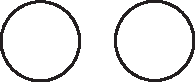
\includegraphics[width=0.2\textwidth]{%
gesamttex/edit_VIII,3/images/LH_37_05_161-162r_d5_162r.pdf%
}} 
\vspace{0.5em}
\centerline{%
\lbrack\textit{Fig.~5}\rbrack%
}
% \newpage%
\vspace{1.5em}
%
%
\pstart 
Si duo corpora aequalia%
\protect\index{Sachverzeichnis}{corpora aequalia} aequali vi%
\protect\index{Sachverzeichnis}{vis} concurrant,%
\protect\index{Sachverzeichnis}{corpora aequalia aequali vi concurrentia} ambo eadem celeritate%
\protect\index{Sachverzeichnis}{celeritas} repelluntur. Si vero major
sit celeritas unius celeritas est permutata.
\pend
\count\Bfootins=1200%
\count\Afootins=1200%
\count\Cfootins=1200